\documentclass[12pt, twoside]{article}
\usepackage[letterpaper, margin=1in, headsep=0.2in]{geometry}
\setlength{\headheight}{0.6in}
%\usepackage[english]{babel}
\usepackage[utf8]{inputenc}
\usepackage{microtype}
\usepackage{amsmath}
\usepackage{amssymb}
%\usepackage{amsfonts}
\usepackage{siunitx} %units in math. eg 20\milli\meter
\usepackage{yhmath} % for arcs, overparenth command
\usepackage{tikz} %graphics
\usetikzlibrary{quotes, angles}
\usepackage{graphicx} %consider setting \graphicspath{{images/}}
\usepackage{parskip} %no paragraph indent
\usepackage{enumitem}
\usepackage{multicol}
\usepackage{venndiagram}

\usepackage{fancyhdr}
\pagestyle{fancy}
\fancyhf{}
\renewcommand{\headrulewidth}{0pt} % disable the underline of the header
\raggedbottom
\hfuzz=2mm %suppresses overfull box warnings

\usepackage{hyperref}

\fancyhead[LE]{\thepage}
\fancyhead[RO]{\thepage \\ Name: \hspace{4cm} \,\\}
\fancyhead[LO]{BECA / Dr. Huson / Geometry\\*  Unit 8: Congruence transformations\\* 9 February 2023}

\begin{document}

\subsubsection*{7.9 Pretest: Mixed congruence transformations \hfill CCSS.HSG.CO.A.5}
\begin{enumerate}
\item Slide $\triangle ABC$ to the right five and up two. Label the image $\triangle A'B'C'$.
\begin{center}
    \begin{tikzpicture}[scale=.7]
    \draw [help lines] (-7,-4) grid (10,6);
    \draw [thick, <->] (-7.4,0) -- (10.4,0) node [right] {$x$};
    \draw [thick, <->] (0,-4.4)--(0,6.4) node [above] {$y$};  
    \draw [thick]
      (-1,2) node[below left] {$A$}--
      (3,-2) node[below] {$B$}--
      (4,1) node[above right] {$C$}--cycle;  
  \end{tikzpicture}
\end{center}

\item Reflect the triangle over the $x$-axis, $\triangle ABC \rightarrow \triangle A'B'C'$. Complete the table of the coordinates and plot and label the image on the grid. \vspace{0.5cm}
  \begin{multicols}{2}
    $A(1,1) \rightarrow$ \\[0.7cm]
    $B(0,4) \rightarrow$ \\[0.7cm]
    $C(4,1) \rightarrow$ \\[0.7cm]
      \begin{tikzpicture}[scale=.75]
      \draw [help lines] (-5,-5) grid (5,5);
      \draw [thick, <->] (-5.4,0) -- (5.4,0) node [right] {$x$};
      \draw [thick, <->] (0,-5.4)--(0,5.4) node [above] {$y$};  
      \draw [thick]
        (1,1) node[below left] {$A$}--
        (0,4) node[above left] {$B$}--
        (4,1) node[below] {$C$}--cycle;  
      \end{tikzpicture}
    \end{multicols}

\newpage
\item A transformation maps $\triangle TOP \rightarrow \triangle CAP$, shown below. 
\begin{enumerate}
  \item Fully specify the transformation. \vspace{1cm}
\begin{multicols}{2}
  \item Identify each corresponding object. 
  \begin{enumerate}
    \item $T \rightarrow$ \rule{2cm}{0.15mm}
    \item $O \rightarrow$ \rule{2cm}{0.15mm}
    \item $P \rightarrow$ \rule{2cm}{0.15mm}
    \item $\angle PTO \cong$ \rule{2cm}{0.15mm}
    \item \rule{2cm}{0.15mm} $\cong \overline {CA}$
  \end{enumerate}
  \begin{tikzpicture}[scale=.48]
    \draw [help lines] (-2,-3) grid (9,8);
    \draw [thick, <->] (-2.4,0) -- (9.4,0) node [right] {$x$};
    \draw [thick, <->] (0,-3.4)--(0,8.4) node [above] {$y$};  
    \draw [thick]
    (4,-2) node[below left] {$C$}--
    (7,1) node[right] {$A$}--
    (1,1) node[below left] {$P$}--cycle;  
    \draw [thick]
    (4,4) node[right] {$T$}--
    (1,7) node[left] {$O$}--
    (1,1) --cycle; 
  \end{tikzpicture}
\end{multicols}
\end{enumerate}

\item Translate $\triangle DEF$ by $(x,y) \rightarrow (x-2, y-5)$, then reflect the result over the $y$-axis. Label the images $\triangle D'E'F'$ and $\triangle D''E''F''$ respectively.
\begin{center}
    \begin{tikzpicture}[scale=.6]
    \draw [help lines] (-7,-5) grid (10,6);
    \draw [thick, <->] (-7.4,0) -- (10.4,0) node [right] {$x$};
    \draw [thick, <->] (0,-5.4)--(0,6.4) node [above] {$y$};  
    \draw [thick]
      (-4,4) node[below left] {$D$}--
      (2,3) node[above] {$E$}--
      (1,1) node[below] {$F$}--cycle;  
  \end{tikzpicture}
\end{center}

\item Check those transformations that are rigid motions.
\begin{itemize}
  \begin{multicols}{2}
  \item[$\square$] Reflection
  \item[$\square$] Dilation
  \item[$\square$] Translation
  \item[$\square$] Rotation
  \item[$\square$] An isometry
  \item[$\square$] Horizontal stretch
  \end{multicols}
\end{itemize}

\end{enumerate}
\end{document}

